\documentclass[12pt,letterpaper]{article}
\usepackage{anysize}
\usepackage{amsmath}
\marginsize{2cm}{2cm}{1cm}{1cm}
\usepackage{listings}
\usepackage{cite}
\usepackage{caption}
\usepackage{upquote}
\usepackage{xcolor}
\usepackage{xcolor}

\usepackage{tikz}
\def\checkmark{\tikz\fill[scale=0.4](0,.35) -- (.25,0) -- (1,.7) -- (.25,.15) -- cycle;} 

\usepackage{graphicx}


\begin{document}

\begin{titlepage}
    \vspace*{4cm}
    \begin{flushleft}
    {\huge
        CS519 Project 5\\[.5cm]
    }
    {\large
        Displacement Mapping and Lighting and Bump Mapping
    }
    \end{flushleft}
    \vfill
    \rule{5in}{.5mm}\\
    Li Li

\end{titlepage}
\section{source files}
There are only three files lab4.frag, lab4.glib and lab4.vert.
\section{a simple explanation}
What I did are:\\
\begin{tabular}{ |l | c |}
  \hline                       
  \textbf{Feature} & \textbf{Status} \\ \hline
  Cos*Cos surface & \checkmark \\ \hline
  Cos*Cos normal & \checkmark \\ \hline
  Extra Credit (normal rotation) & \checkmark \\ \hline
\end{tabular}

\begin{itemize}
\item For the this \textbf{Cos*Cos surface} it is not very difficult. The x and y value of each vertex would remain the same, only z value we need to make a difference. I made it just as the function given in the project $Z = A * cos(Bx) * cos(Cy)$. 
\item Now when compute \textbf{Normal of these new vertexes}. I compute the 2 calculus derivatives vector that travels two direction which are on the plane of the calculus surface. And in this case, we can normalize the corss product of them to obtain normal of this vector.
\item About \textbf{lighting}, it is pretty much what lighting shader did. I just want to mention that "flat in vec3 vNf" confuse me in the beginning. I don't know why I need to add this flat. After trying comment it out and I figure out it just prevent interpolate normals. And give just one normal to one primitive.
\item Finally, for \textbf{extra credit}. Noise is similar to previous project, but I did \textit {angx = angx*$\pi$;} I modified range from  $-\pi$ to $\pi$. That is because I believe this angle range can cover all possibilities. All of this noise work is done in vertex shader. vMC would be my new\_vertex which is created in \textbf{Cos*Cos surface} step.
\end{itemize}
\section{result}

\begin{figure}[p]
    \centering
    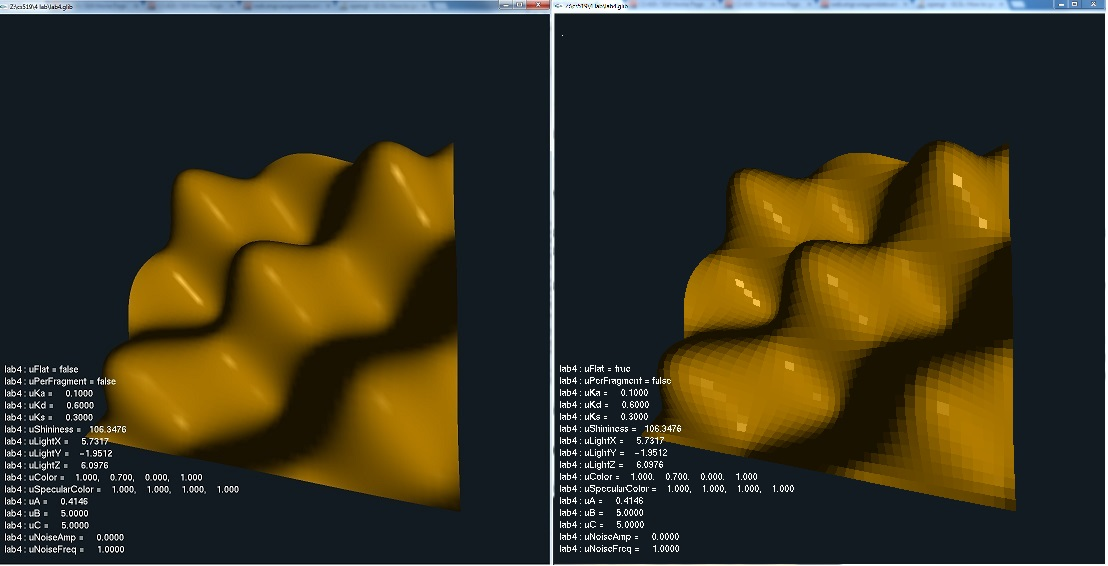
\includegraphics[width=1.0\textwidth]{1.jpg}
    \caption{smooth shading(left) and flat shading}
\end{figure}

\begin{figure}[p]
    \centering
    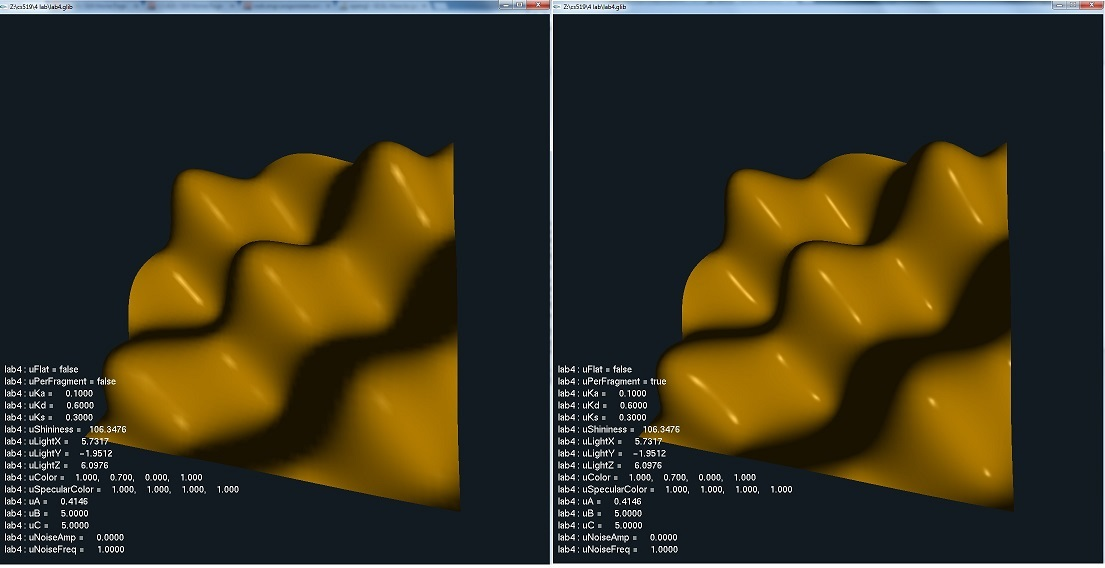
\includegraphics[width=1.0\textwidth]{2.jpg}
    \caption{per-vertex lighting(left) and per-fragment}
\end{figure}

\begin{figure}[p]
    \centering
    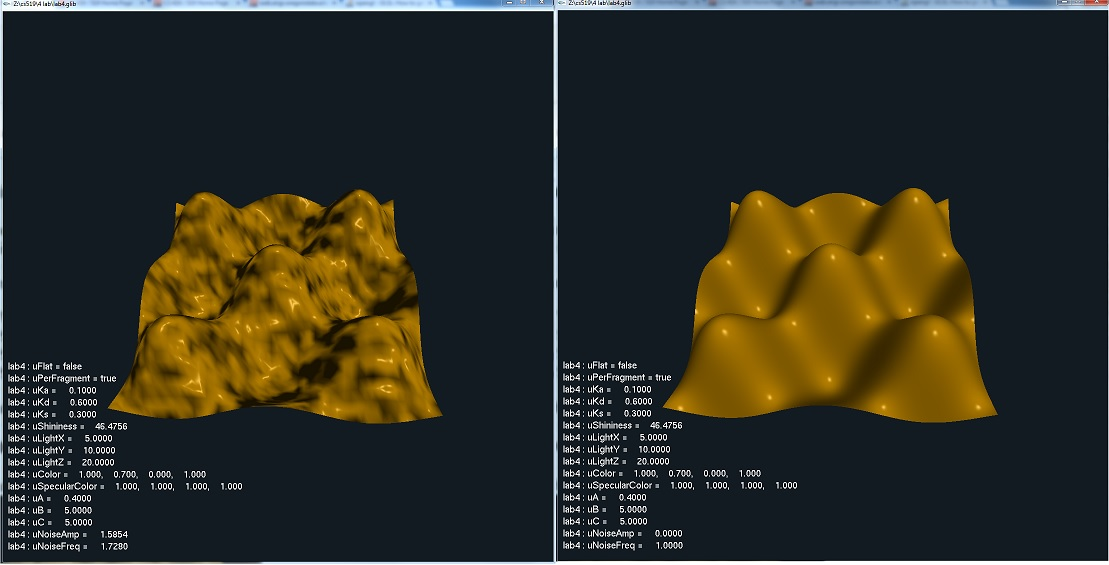
\includegraphics[width=1.0\textwidth]{3.jpg}
    \caption{bump-mapped(left) and not bump-mapped}
\end{figure}

\end {document}
